Since the neural network topologies between the backends are shown to be similar,
the parameters related to this topology are shared as well.
By applying the theory from \textcite{Rueckauer2017} (see section
\ref{sec:coding}), this section will explain how input data, network weights,
and network biases can be transferred from \glspl{ANN} to \glspl{SNN}.
It will then proceed to describe the setup with which prepares the scene for the
experimental results in the following chapter.

As explained in Section \ref{sec:coding}, normalised input in \glspl{ANN} can
be inserted into \glspl{SNN} with the help of a linear transformation.
This transformation has been examined empirically, by constructing a simple 
one-neuron network, and injecting a constant current over time.
By running a number of experiments, it is possible to measure the integrated
current in the neuron and the amount of spikes it produces over time.

\begin{figure}
  \centering
  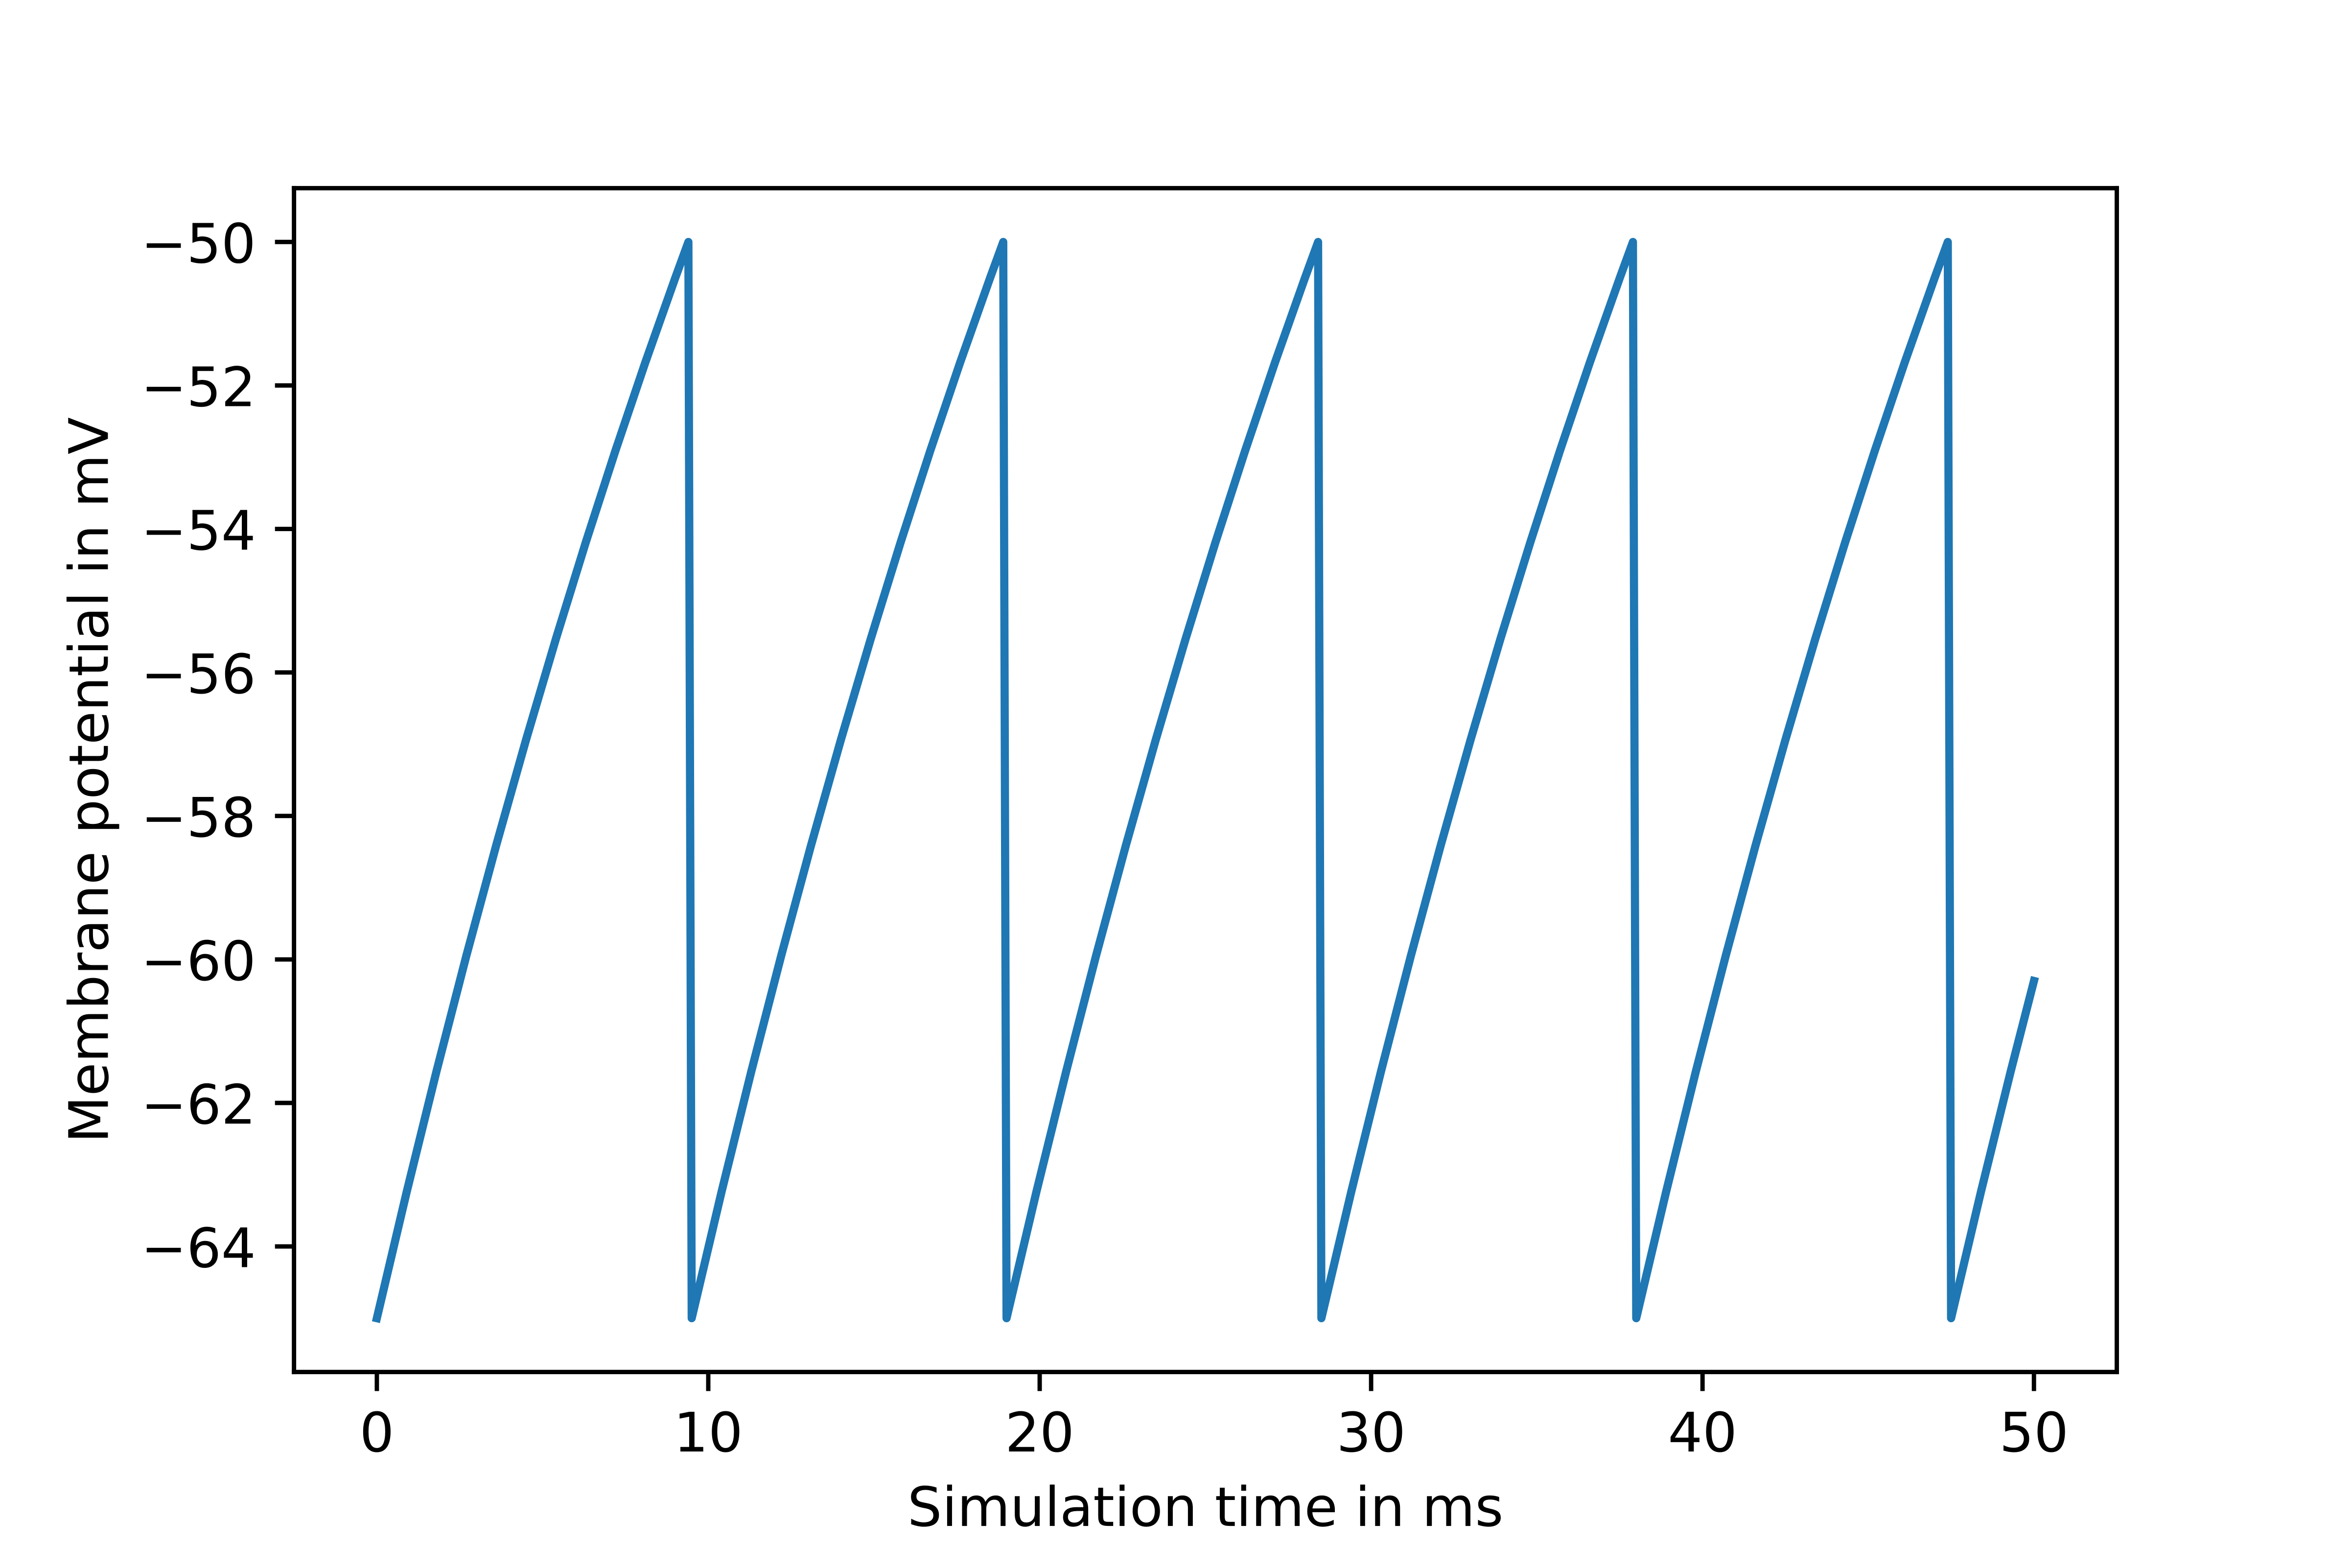
\includegraphics[width=0.8\textwidth]{images/membrane.png}
  \caption{Membrane potential for a LIF neuron given a constant input current of
  2 nA, simulated over 100 ms.}
  \label{fig:membrane}
\end{figure}

Figure \ref{fig:membrane} shows one such experiment, in which the membrane
potential of a single neuron is plotted over time.
The neuron is given a constant input current of 1.3 nA, and 
produces 5 spikes during the 100 ms simulation time. 
As expected in section \ref{sec:coding}, the interspike interval is constant.

A neuron only spikes when its membrane potential exceeds its excitation threshold
$V_{thr}$, but depends on a number of parameters to describe the neuron
conductivity, current decay time etc.
In ll three, PyNN, NEST and BrainScaleS, these parameters can be programatically
defined. Table \ref{tab:neuron_parameters} shows the default parameters for
NEST (also shown in Listing \ref{lst:lif-cond-exp}).
The $\tau_{syn}$ parameters denote the decay time for the input spike currents. 
Similarly, the membrane time constant, $\tau_m$, expresses the time it takes for the
neuron membrane to decay to its resting state ($V_{rest}$) if no other
input arrives. 
For the LIF\index{neuron model!leaky-integrate-and-fire} model used in PyNN,
all $\tau$ parameters decay exponentially \cite{Davison2009}.
The $V_{rev}$ parameters explain the potential to integrate into the neuron,
when either excitatory or inhibitory input arrives. 

\renewcommand{\arraystretch}{1.3} 
\begin{table}
\begin{tabular}[center]{l r l l}
  \hline
  $C_m$ & 1 & nF & Capacity of the membrane. \\ \hline
  $I_{offset}$ & 0 & nA & Offset current. \\ \hline
  $V_{rest}$ & -65 & mV & Resting membrane potential. \\ \hline
  $V_{reset}$ & -65 & mV & Reset potential after a spike. \\ \hline
  $V_{rev}^E$ & 0 & mV & Reverse potential for excitatory input. \\ \hline
  $V_{rev}^I$ & -70 & mV & Reverse potential for inhibitory input. \\ \hline
  $V_{thr}$ & -50 & mV & Spike threshold. \\ \hline
  $\tau_m$ & 20 & ms & Membrane time constant. \\ \hline
  $\tau_{refrac}$ & 0.1 & ms & Duration of the refractory period. \\ \hline
  $\tau_{syn}^E$ & 5 & ms & Decay time of the excitatory synaptic conductance. \\ \hline
  $\tau_{syn}^I$ & 5 & ms & Decay time of the inhibitory synaptic conductance. \\  \hline
\end{tabular}
\caption{The names, default values and description of the neuron parameters in
PyNN, NEST and BrainScaleS.}
\label{tab:neuron_parameters}
\end{table}

With the exception of $I_{offset}$, which is the constant input current,
the parameters are kept constant in Volr, and used in all spiking backends
to avoid spurious influences.
